\pdfminorversion=4
\documentclass[aspectratio=169]{beamer}

\mode<presentation>
{
  \usetheme{default}
  \usecolortheme{default}
  \usefonttheme{default}
  \setbeamertemplate{navigation symbols}{}
  \setbeamertemplate{caption}[numbered]
  \setbeamertemplate{footline}[frame number]  % or "page number"
  \setbeamercolor{frametitle}{fg=white}
  \setbeamercolor{footline}{fg=black}
} 

\usepackage[english]{babel}
\usepackage{inputenc}
\usepackage{tikz}
\usepackage{courier}
\usepackage{array}
\usepackage{bold-extra}
\usepackage{minted}
\usepackage[thicklines]{cancel}
\usepackage{fancyvrb}
\usepackage{setspace}

\xdefinecolor{dianablue}{rgb}{0.18,0.24,0.31}
\xdefinecolor{darkblue}{rgb}{0.1,0.1,0.7}
\xdefinecolor{darkgreen}{rgb}{0,0.5,0}
\xdefinecolor{darkgrey}{rgb}{0.35,0.35,0.35}
\xdefinecolor{darkorange}{rgb}{0.8,0.5,0}
\xdefinecolor{darkred}{rgb}{0.7,0,0}
\definecolor{darkgreen}{rgb}{0,0.6,0}
\definecolor{mauve}{rgb}{0.58,0,0.82}

\title[2022-09-28-future-trends-python]{Status of Analysis --- The Python Perspective}
\author{Jim Pivarski}
\institute{Princeton University -- IRIS-HEP}
\date{September 28, 2022}

\usetikzlibrary{shapes.callouts}

\begin{document}

\logo{\pgfputat{\pgfxy(0.11, 7.4)}{\pgfbox[right,base]{\tikz{\filldraw[fill=dianablue, draw=none] (0 cm, 0 cm) rectangle (50 cm, 1 cm);}\mbox{\hspace{-8 cm}
\includegraphics[height=1 cm]{princeton-logo-long.png}\hspace{0.1 cm}\raisebox{0.1 cm}{
\includegraphics[height=0.8 cm]{iris-hep-logo-long.png}}\hspace{0.1 cm}}}}}

\begin{frame}
  \titlepage
\end{frame}

\logo{\pgfputat{\pgfxy(0.11, 7.4)}{\pgfbox[right,base]{\tikz{\filldraw[fill=dianablue, draw=none] (0 cm, 0 cm) rectangle (50 cm, 1 cm);}\mbox{\hspace{-8 cm}
\includegraphics[height=1 cm]{princeton-logo.png}\hspace{0.1 cm}\raisebox{0.1 cm}{
\includegraphics[height=0.8 cm]{iris-hep-logo.png}}\hspace{0.1 cm}}}}}

% Uncomment these lines for an automatically generated outline.
%\begin{frame}{Outline}
%  \tableofcontents
%\end{frame}

% START START START START START START START START START START START START START

\begin{frame}{Something I want to address in this talk}
\vspace{0.1 cm}
\begin{center}
\only<1>{
\includegraphics[width=0.85\linewidth]{PLOTS/indico-future2022.png}}\only<2>{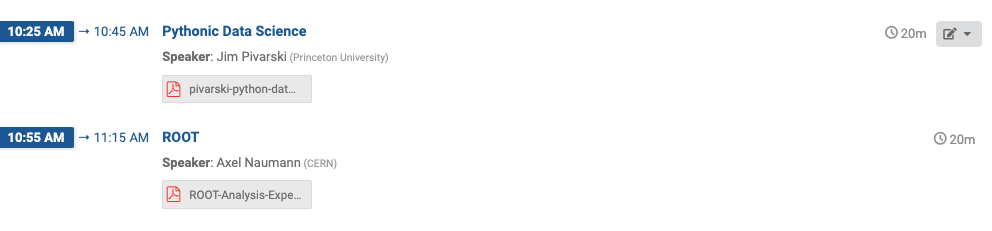
\includegraphics[width=0.85\linewidth]{PLOTS/indico-hllhc2021.png}}\only<3>{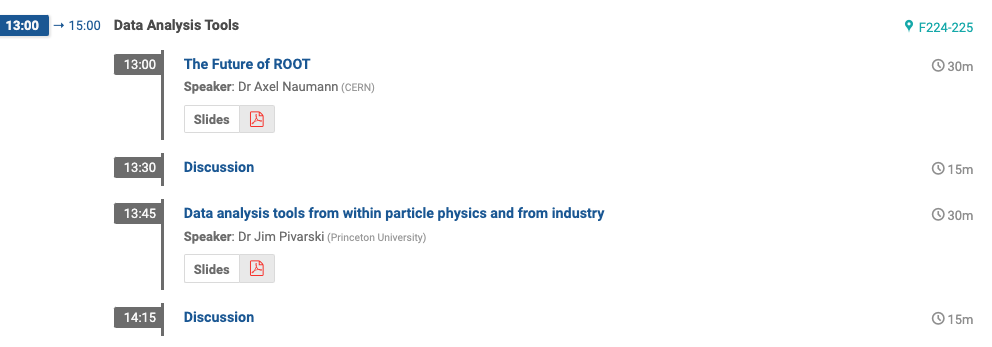
\includegraphics[width=0.85\linewidth]{PLOTS/indico-roundtable2018.png}}\only<4>{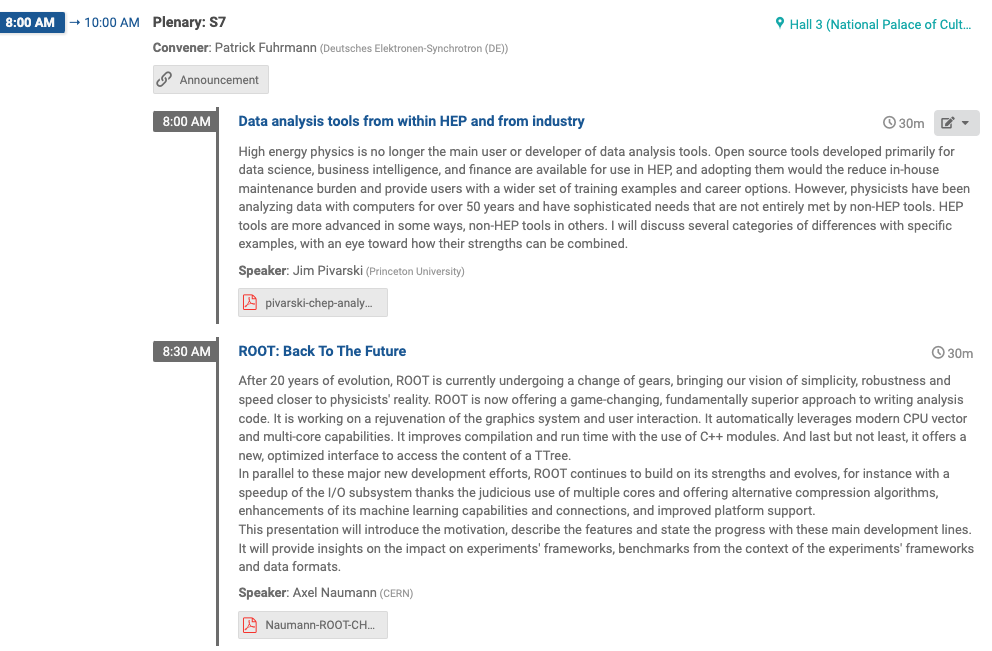
\includegraphics[width=0.85\linewidth]{PLOTS/indico-chep2018.png}}
\end{center}
\end{frame}

\begin{frame}{\mbox{ }}
\Large
It might be an efficient way to summarize all the analysis activities:
\begin{center}
Python $\bigcup$ ROOT.
\end{center}

\vspace{1 cm}
\uncover<2->{But sometimes people read into it an implicit ``versus.''}
\end{frame}

\begin{frame}{\mbox{ }}
\Large
\vspace{0.25 cm}
ROOT has had a Python interface since 2004.

\vspace{0.2 cm}
\begin{itemize}
\item<2-> PyROOT is old enough to vote!
\end{itemize}

\vspace{1.25 cm}
\begin{uncoverenv}<3->
Nor is the alternative strictly ``Python.''
\vspace{0.2 cm}
\begin{itemize}
\item<4-> I've also tried to characterize it as ``industry'' or ``data science.''
\end{itemize}
\end{uncoverenv}
\end{frame}

\begin{frame}{\mbox{ }}
\Large
What we're trying to talk about here is a social trend, and we're using a programming language as a proxy for it.
\end{frame}

\begin{frame}{Analysis of 11\,635 GitHub repos created by 2\,172 CMS physicists}
\vspace{0.25 cm}

Software for the CMS experiment is on GitHub and only CMS physicists need to fork it. Using that, we can examine all of those physicists' non-fork, public repositories.

\vspace{0.2 cm}

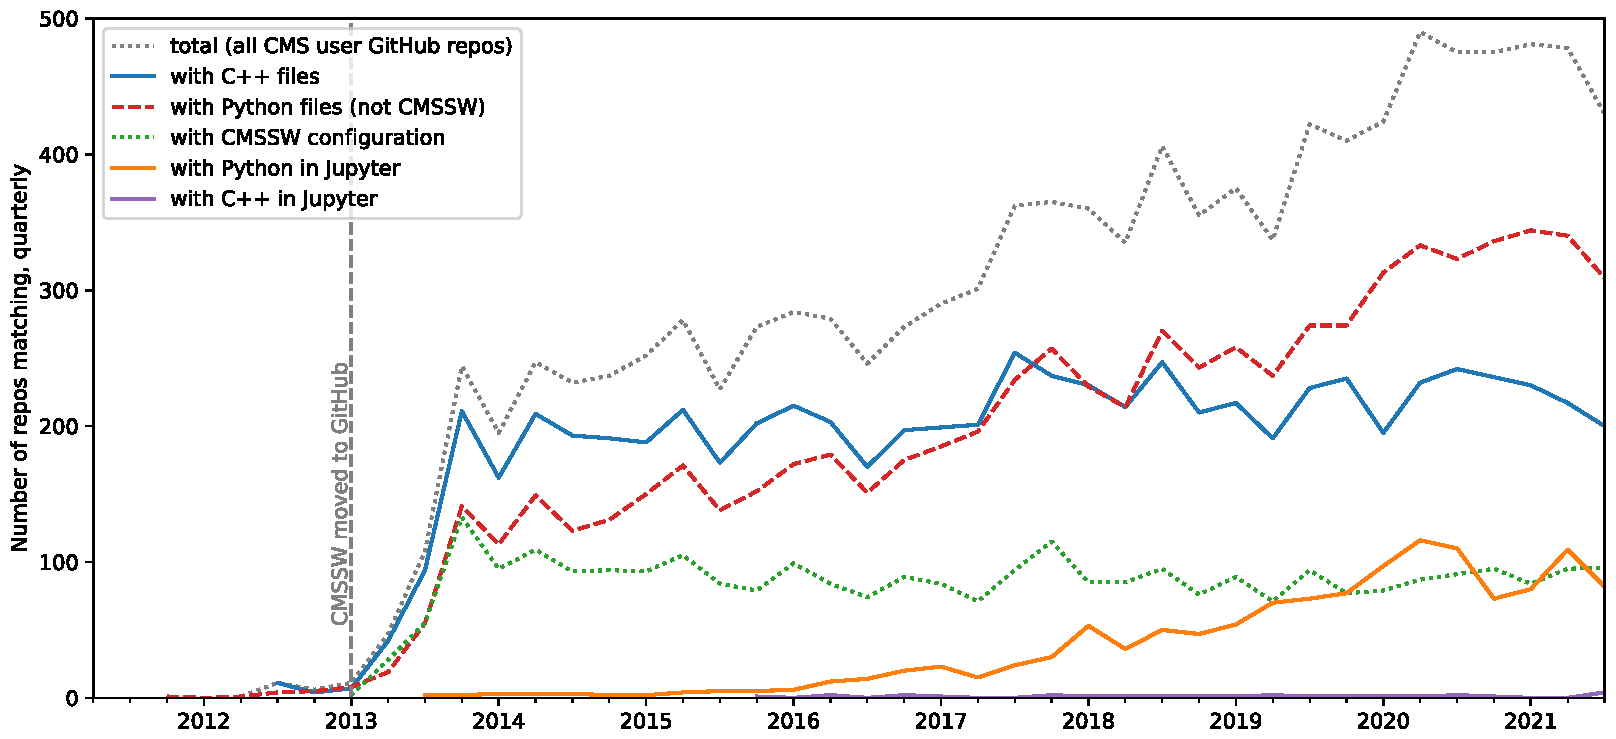
\includegraphics[width=\linewidth]{PLOTS/gihub-language-fullstudy.pdf}
\end{frame}

\begin{frame}{Analysis of 11\,635 GitHub repos created by 2\,172 CMS physicists}
\vspace{0.25 cm}

By regex searching for ``\mintinline{python}{import [A-Za-z_][A-Za-z_0-9]*}'' etc., we can count the number of physicist repositories that use different packages over time.

\vspace{0.2 cm}

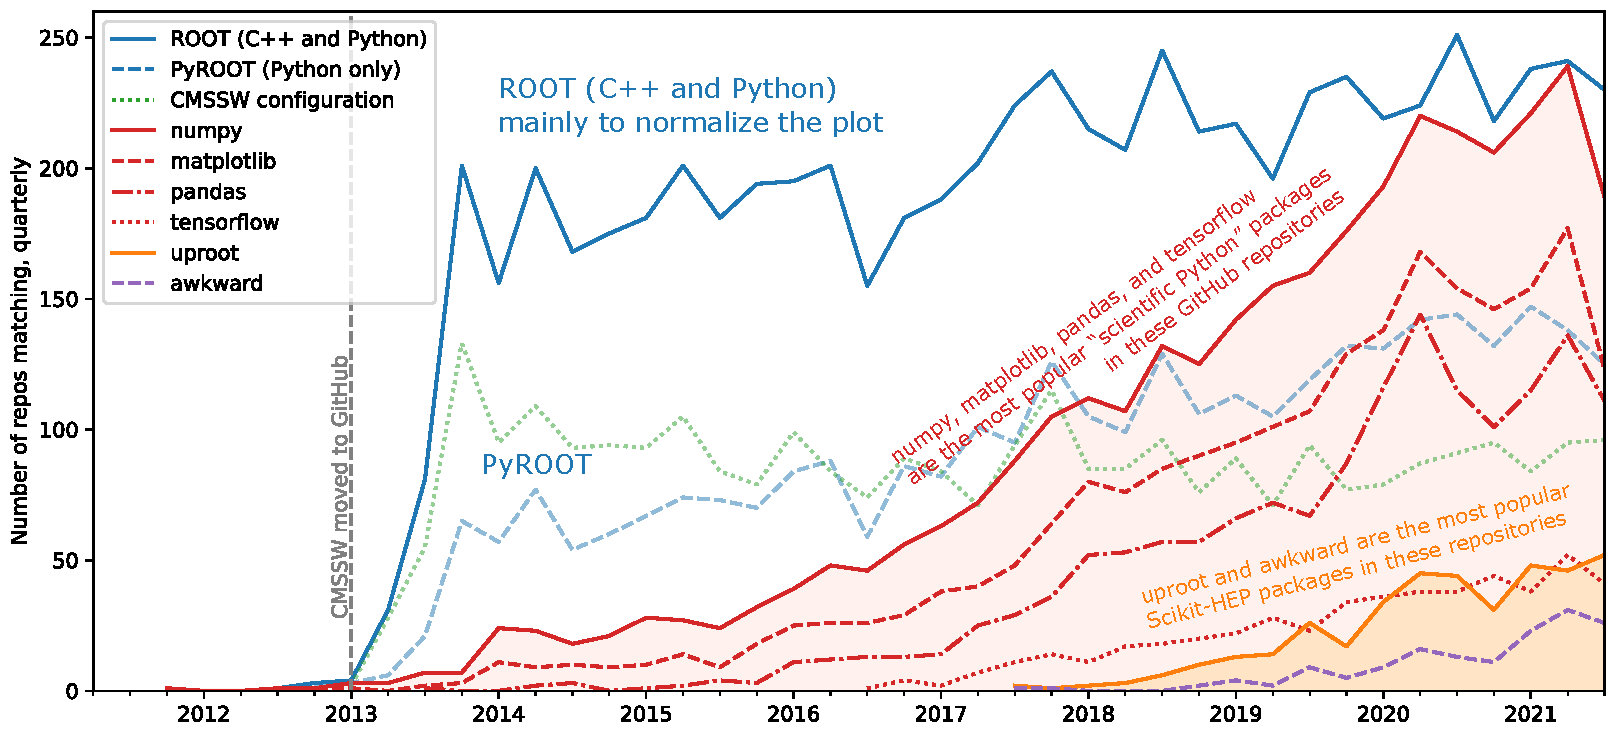
\includegraphics[width=\linewidth]{PLOTS/gihub-package-fullstudy.pdf}
\end{frame}

\begin{frame}[fragile]{\mbox{ }}
\Large
There is a rise in Python usage (including PyROOT).

\vspace{1.5 cm}
\begin{uncoverenv}<2->
But the biggest thing that happened in the past 5 years is

\begin{center}
\begin{minipage}{3.5 cm}
\begin{minted}{python}
import numpy
\end{minted}
\end{minipage}
\end{center}

\vspace{0.2 cm}
\begin{spacing}{1.0}
What we're really seeing is the use of data analysis tools developed by scientists from other fields, the Big Data industry, quants, \dots
\end{spacing}
\end{uncoverenv}
\end{frame}

\begin{frame}{In fact, Python, the language, has been in HEP for a long time}
\vspace{0.25 cm}

Regex matches to all Computing in High Energy Physics (CHEP) titles and abstracts.

\vspace{-0.1 cm}
\begin{center}
\only<1>{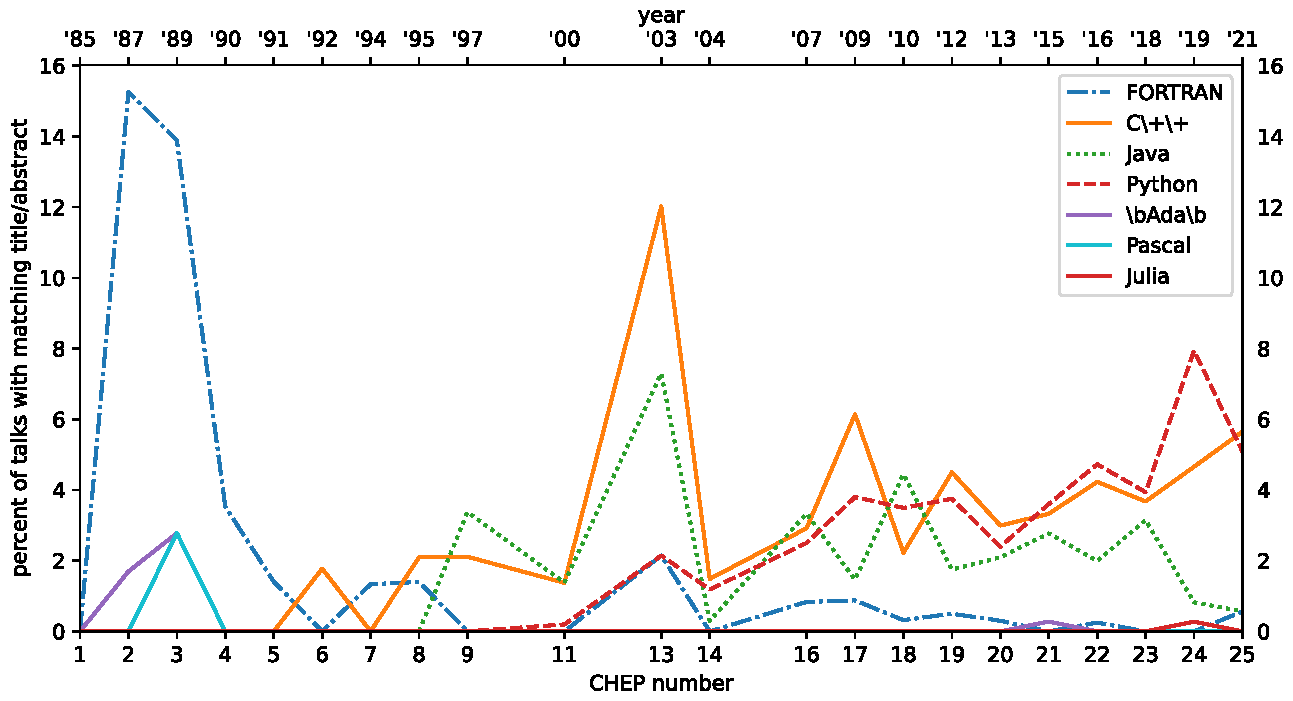
\includegraphics[width=0.95\linewidth]{PLOTS/chep-papers-language.pdf}}\only<2>{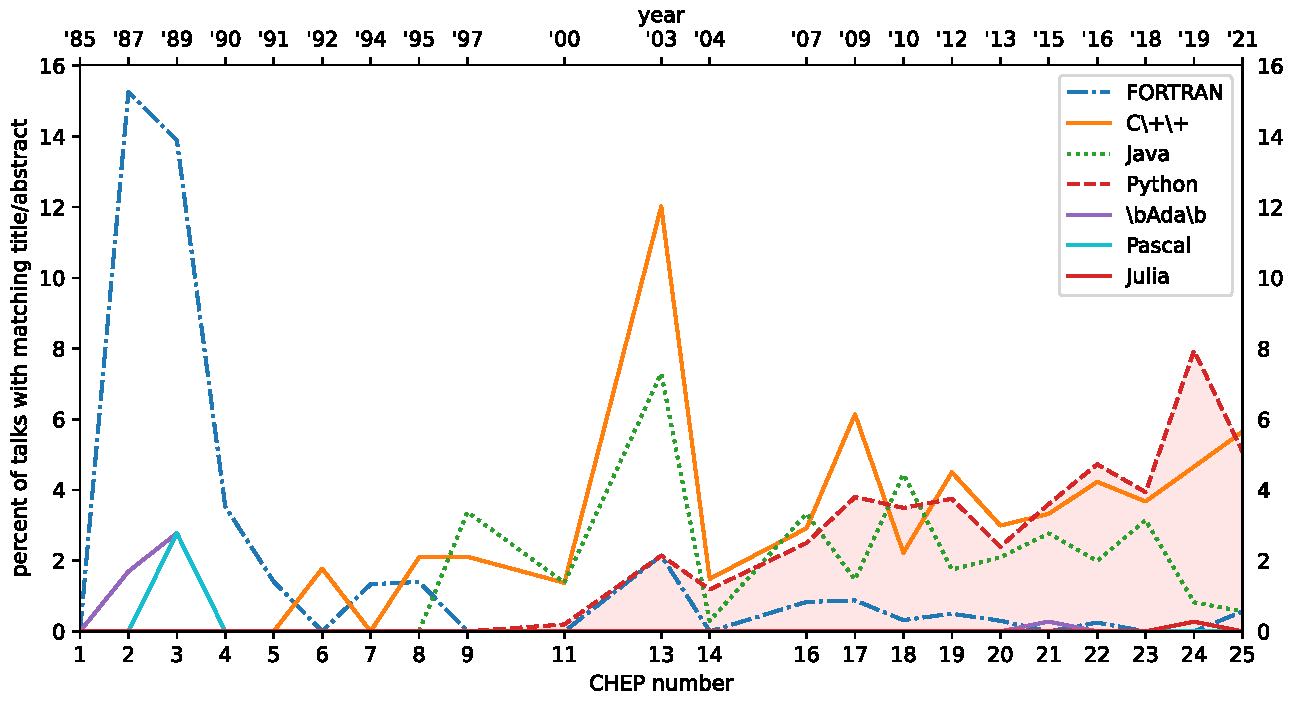
\includegraphics[width=0.95\linewidth]{PLOTS/chep-papers-language-shaded.pdf}}
\end{center}
\end{frame}

\begin{frame}{Lucas Taylor, summary of data analysis track, CHEP 2001}
\vspace{0.25 cm}

\mbox{ } \hfill 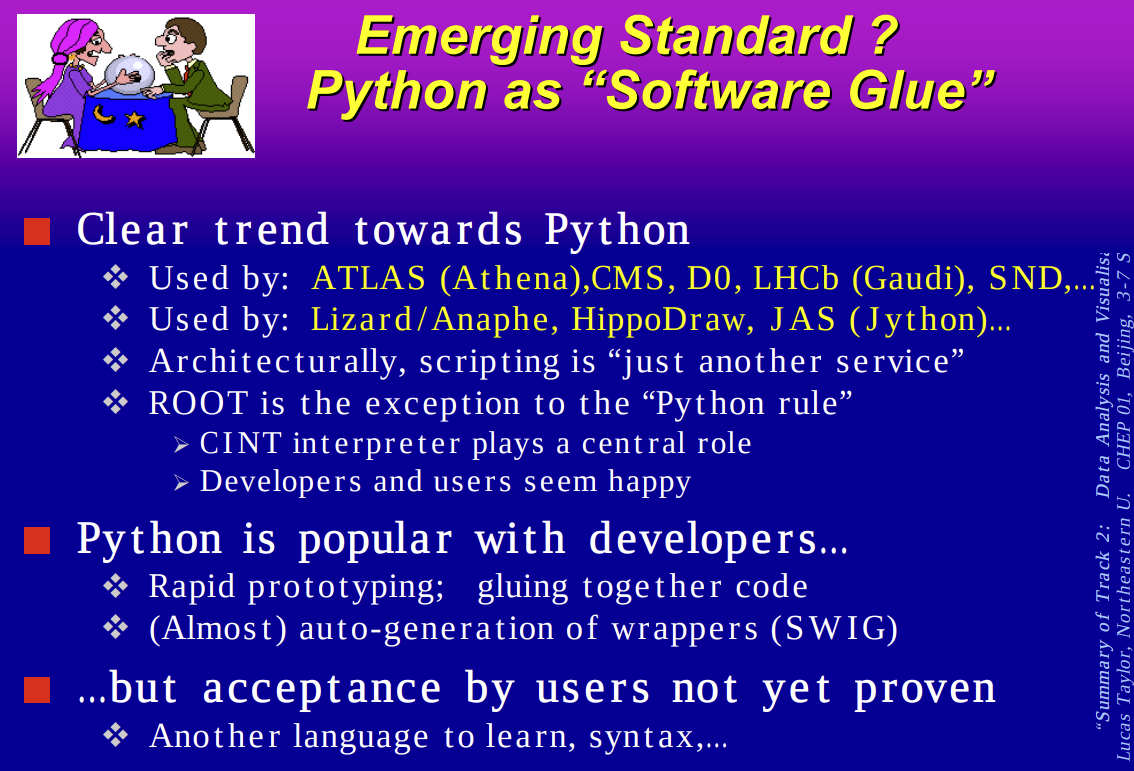
\includegraphics[width=0.82\linewidth]{PLOTS/chep-2001-python.png} \hfill \mbox{ }
\end{frame}

\begin{frame}{The {\it change} is likely driven by machine learning}
\vspace{0.25 cm}

Regex matches to all Computing in High Energy Physics (CHEP) titles and abstracts.

\vspace{-0.1 cm}
\begin{center}
\only<1>{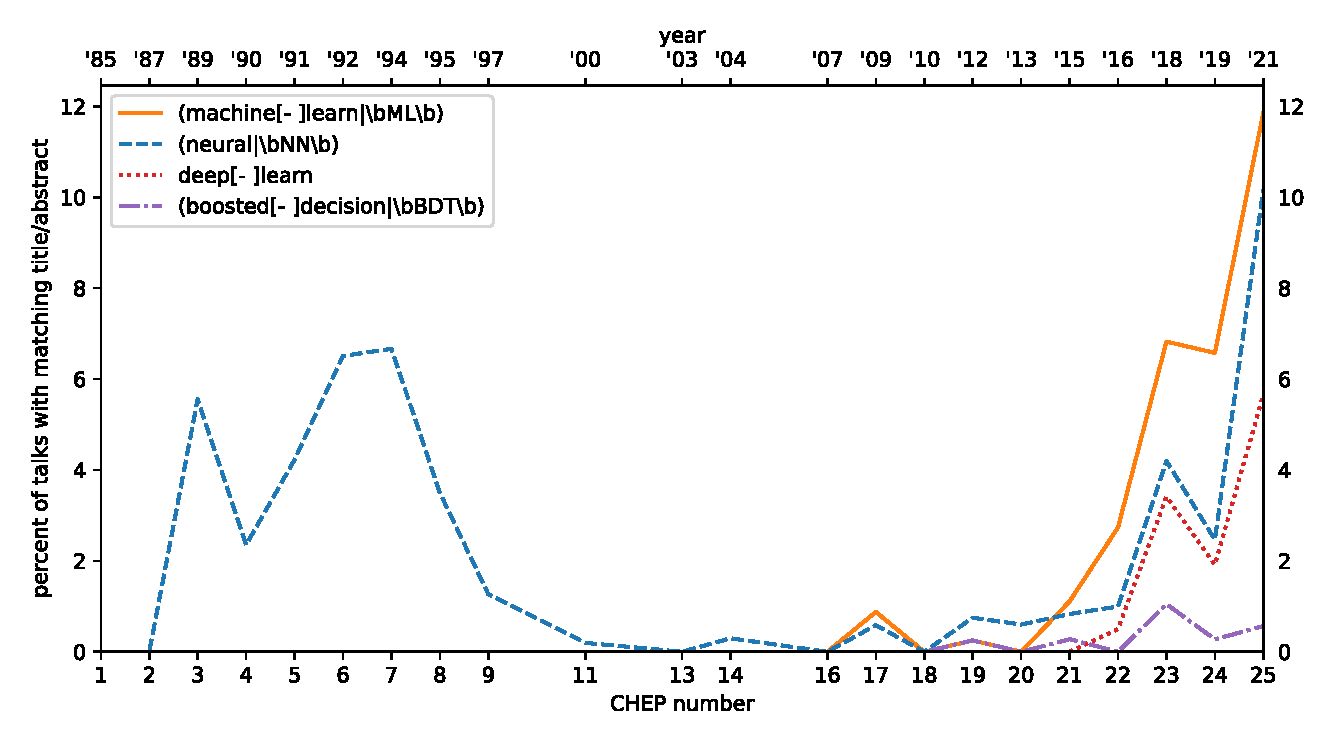
\includegraphics[width=0.95\linewidth]{PLOTS/chep-papers-ml.pdf}}\only<2>{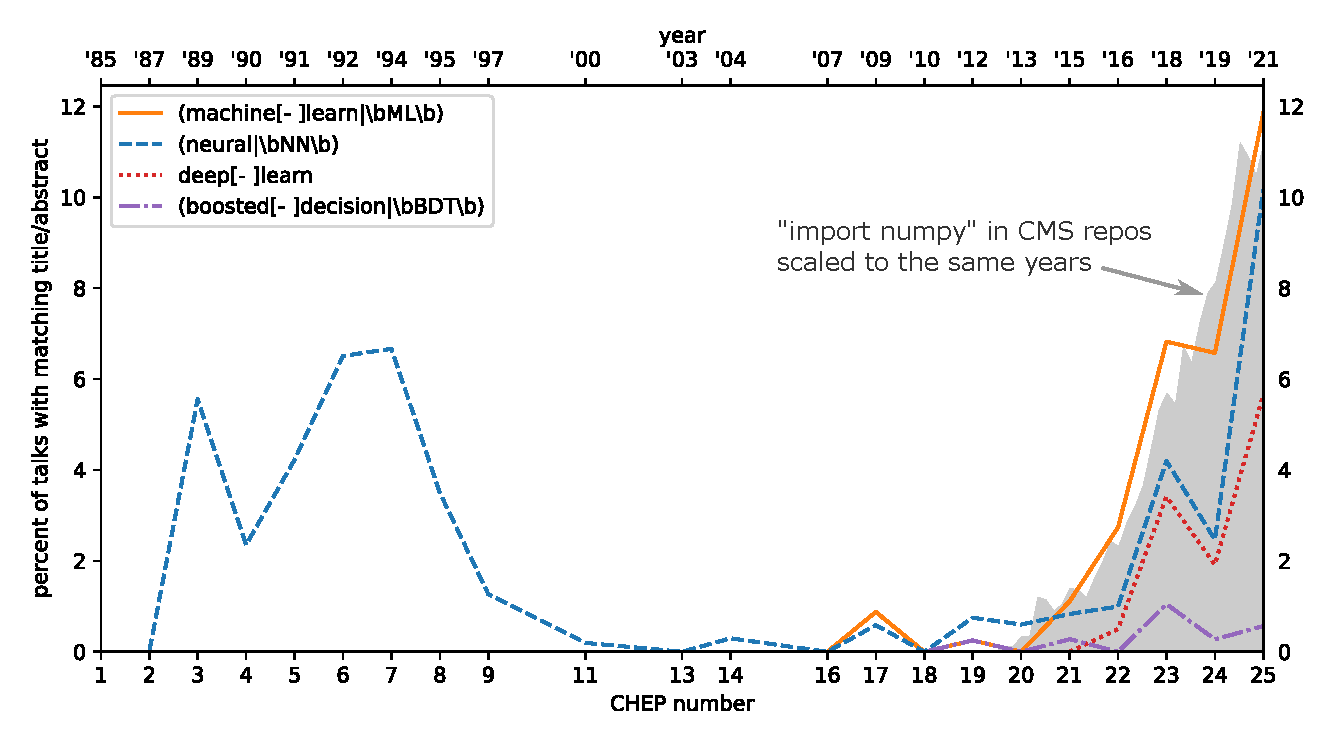
\includegraphics[width=0.95\linewidth]{PLOTS/chep-papers-ml-explained.pdf}}
\end{center}
\end{frame}

\begin{frame}{PyHEP 2020 survey}
\vspace{0.5 cm}
\begin{columns}
\column{1.1\linewidth}
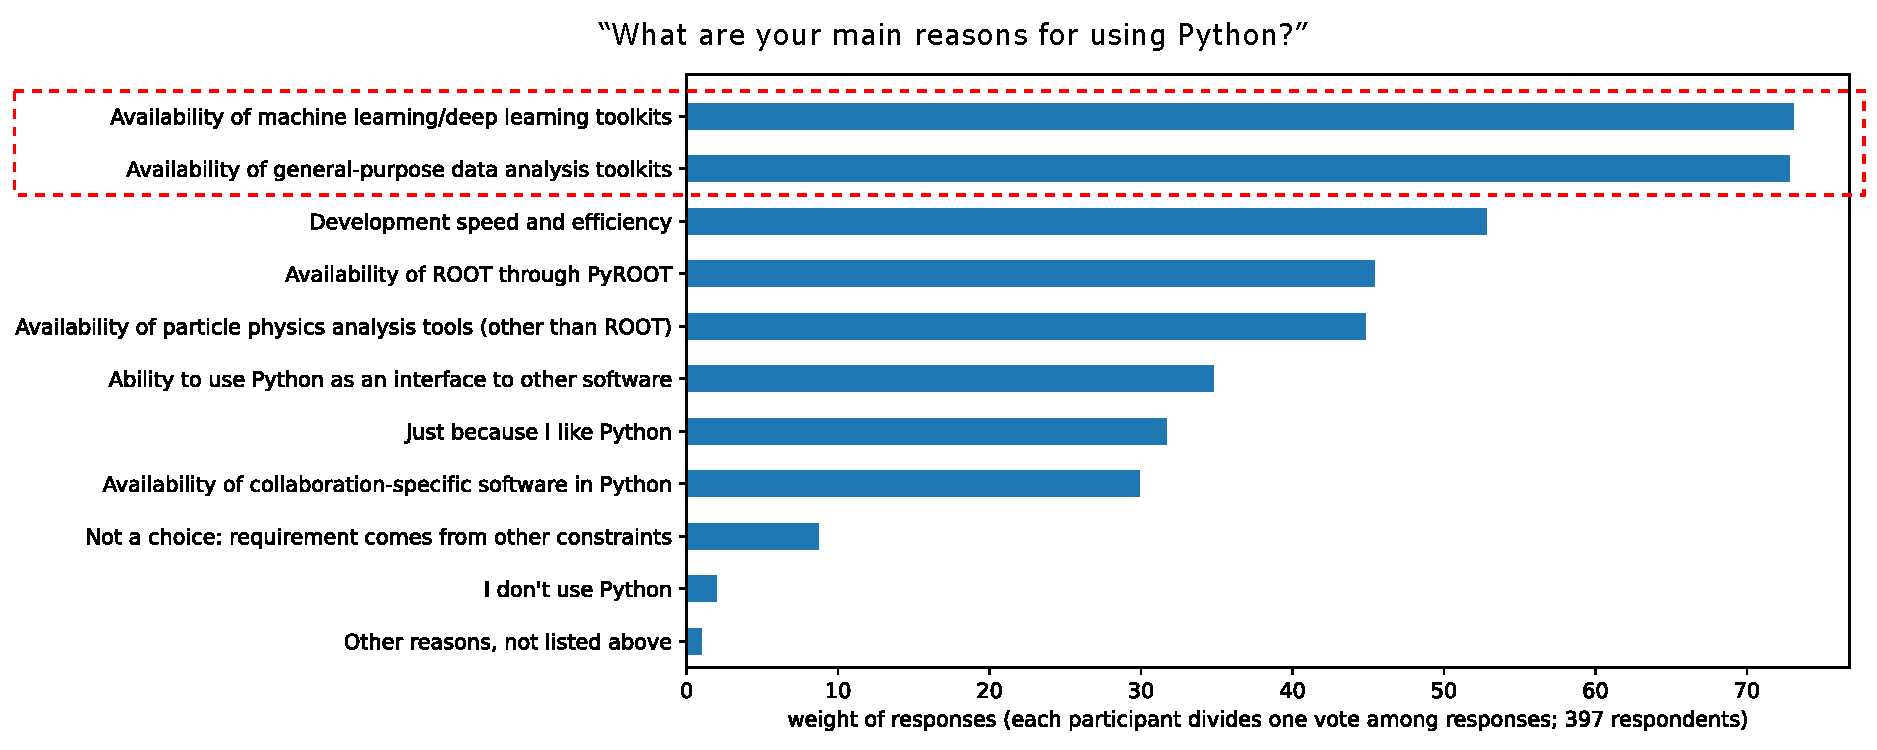
\includegraphics[width=\linewidth]{PLOTS/pyhep2020-why-use-python.pdf}
\end{columns}
\end{frame}




\end{document}
